\documentclass{article}

\usepackage[utf8]{inputenc}
\usepackage[danish]{babel}
\usepackage{float}
\usepackage{fancyhdr}
\usepackage{amsmath}
\usepackage{color}
\usepackage{listings}
\usepackage{graphicx}
\usepackage{lastpage}
\usepackage{enumitem}
\usepackage[a4paper, top = 1in, bottom = 1in, left=1in,right=1in]{geometry}
\usepackage{tikz}
\usepackage{tikz-qtree}
\usepackage{listingsutf8}

\title{Human Computer Interaction}
\author{Peter Heilbo Ratgen}
\date{\today, 1. semester}


\begin{document}
\maketitle

\section{Undervisning 15. september}
\subsection{Opsamling på øvelsestimer} 
Sprint questions, skal mest dreje sig om projektet, og ikke så meget om
management spørgsmål som fx "hvordan kan vi finde funding?".
Kurset handler om at skabe ideer i den rigtige retning, vi skal ikke vide hvad
prprojektet ender som. Alle artefakter skal omhandle brugerens rejse.

\subsection{Sketching}
Er en visuel måde at brainstorme på. Det er ikke mening at det skal være pænt.
Pointen er at give et overblik. Alle folk kan sketche. En sketch er primært
firkanter, cirkler og streger og måske et ord. Et billede siger mere end 1000
ord. 
Det er vigtigt at tegne for at starte tankeprocesser. Det er også med til at
give et fælles overblik. Det er bedst at sketche på papir eller et whiteboard.
Pointen er at holde det basic med papir og blyant, lige så snart man involverer
teknologi, giver man en barrier-of-entry så en kunde kunne finde på ikke at
bidrage.

\subsection{Design sprint}
\paragraph{Lightning demos} Vi laver en liste af demo system kandidater. Vi
skriver 1-2 systermer og skriver dem på whiteboardet. Vi skal give hinanden en 3
minutters demo, hvor man starter med overall system og dykker ned i enkelt
særlige detaljer.

\begin{itemize}
  \item Noter
  \item Ideer
  \item Crazy 8s
    \subitem En god måde at give hjernen en løbetur på. Man deler papiret i 8 og
    laver 8 sketches på 8 minutter.
  \item Præsenter dine sketches
    \subitem Hver person præsenterer sine sketches. Vi vil gerne tale om vores
    ideer.
  \item Iterér 
    \subitem Nu har vi set nogle forskellige ting, så kan vi få nye ideer.
\end{itemize}

Bagefter trækker vi linjer mellem de forskellige komponenter. Således at vi kan
flytte rundt på komponenterne.

\newpage
\section{Undervisning 29. September}
\subsection{Opsamling}
Husk at sende ham en mail med arbejdet efter hver instruktortime. Der kommer en
rapport til aflevering, omhandlende design-sprintet.

\subsection{Onsdag}

Ideerne skal præsenteres af en anden. Dvs. at hver skal komme med deres egen
sketch. Vi laver et heatmap med dotvoting for de elementer vi bedst kan lide.
Beslutningerne skal laves af beslutteren, her er demokrati ikke nødvendigvis det
bedste.
Med en Rumble laver man flere forskellige prototyper for at teste flere
varianter af på brugere.

\paragraph{Storyboard} 
Vi skal være specifikke i hvad brugerens rejse er. Det første er uden for
systemet, fx hvordan man kommer ind i systemet. I den sidste firkant er, hvordan
brugeren er færdig med vores system.

Hver prototype skal have et navn. Når vi skal teste brugeren, skal de to
præsenteres for to forskellige systemer, da kunne man spørge "hvilket system
kunne du bedst tænke dig at anvende i fremtiden?". Det skal ikke være navnet på
det endelige system. Et dårligt navn kan være nok
til at brugeren får et dårligere indtryk af prototypen.

Hvad gør man når man ikke kan få et .com domæne. Kort sagt så skal man være
kreativ.

\newpage

\section{Undervisning 06. Oktober - Prototyping}

\paragraph{Catchup}
Ændret semesterplan, der kommet noget mere på omkring modern UI. De indsendte
storyboards ser fine ud.

\paragraph{Prototyper}
En prototype er den første version, det er det absolut mindste der kan testes.
Det ligger inden et Proof of Concept eller et Minimum Viable Product.
Pretotyping kan man også kalde det allermindste testbare produkt. Fail fast, for
at finde ud af om det man arbejder på er skidt.

Man kan bruge noget der hedder POP, prototyping on paper. Man kan også lave
prototyper i KeyNote og PowerPoint. Her kan man download templates til at
anvende i PowerPoint, så man skal ikke bruge de indbyggede figurer.
Vi skal anvende Figma, her får vi en testbar side. Så man kan hurtig få en
illusion af man faktisk bruger en app. Figma har indbygget vektorgrafik, måden
af arbejde ligner lidt at lave UI til Android eller iOS.

\paragraph{Figma}
\begin{itemize}
  \item Opret en frame til en bestemt device.
  \item Man kan så tegne på hvert et frame, fx skrive tekst, størrelse.
  \item For at lave knap laver man en boks. I venstre side er der en liste over
    de forskellige elementer i tegningen.
  \item Går over i create component for at gøre fx en boks til et objekt. Da kan
    man ændre i alle instances af et objekt.
  \item Man kan trække en pil fra de for forskellige kasser, så man kan linke
    til andre sider.
  \item Linket man får kan man bare sende linket videre, fx kan man bruge det på
    en telefon.
  \item Man kan også anvende vektorgrafik.
\end{itemize}

Det er en dårlig idé at kun at skrive email og password som hints, således at de
forsvinder når man skriver.

Man kan også anvende bootstrap studio. Her kan man bygge hele frontends, det her
er lidt over prototypestadiet. Det er det man kan kalde en codeready prototype.


\newpage
\section{Testing - 27. Oktober} 
Det er vigtigt at kunne se brugerens ansigt når man tester. Man kan enten bruge
et kamera der står og optager imens brugeren testes, der kan også bruges
videoopkald. Her er det vigtigt at der er video på opkaldet. Her er det også
vigtigt at der bliver optaget, således at testen kan bruges efterfølgende.
Vi bruger en halv time på hver test. 

\begin{itemize}
  \item Det er vigtigt at byde velkommen, på en god måde og at fortælle hvad
    testen skal handle om.
  \item Når vi stiller spørgsmål, skal det være enkelte åbne spørgsmål. Det skal
    gerne være enkelt hv-ord, og det er vigtigt at vi ikke svarer på vegne af
    brugeren.
  \item The Five Dysfunctions of a Team, brugere kan selv komme med gode svar
    når man lader dem tænke selv, måske selv efter et halvt minut. 
  \item Introduktion til prototypen, hvad er prototypen, hvad går det ud på. Vi
    kan hive fat i et persona. 
  \item Opgaven - vi skal huske at præsentere hele opgaven i starten, om det er
    1, 2 eller 3 prototyper brugeren skal teste.
  \item Det vigtigt at selve testen skal optages. Vi skal lade være med at være
    eksperter omkring vores prototype. Brugeren skal selv udforske prototypen.
    Hold brugeren talende, "hvorfor klikkede du der?", "kan du bruge den her
    flade til noget", mv.
  \item Debriefing
  \item Kvantificering af problempunkter. 
  \item Pitfalls
    \subitem Vi skal lade være med at spørge til ting som andre syntes er træls.
    Vi skal give mål til brugeren, ikke vise dem hvad produktet går ud på.
\end{itemize}

\newpage
\section{Graphic Design - 3. November} 
Hvordan laver noget der er æstetisk og pænt. Noget der er æstetisk er ikke
nødvendigvis pænt. Der er også noget omkring forventninger der skal stemme
overens med brugeren, således at siden ikke virker utroværdig. Fx Candy
Crush-grafik går ikke til en hjemmeside for rutschebaner.
Øjet kan nemt snydes, fx med linjer der er lige lange, men ikke ligner de fordi
de afsluttes forskelligt. Man kan bruge paletton.com til at finde farver. 

Skeumorphism er at vi bruger udtryk som 'skrivebord', 'mappe' om emner på en
grafisk brugergrænseflade. Et godt eksempel er det gamle iOS, det har man senere
ændret fordi man mente at folk havde godt nok kendskab.

\begin{figure}
  \centering
  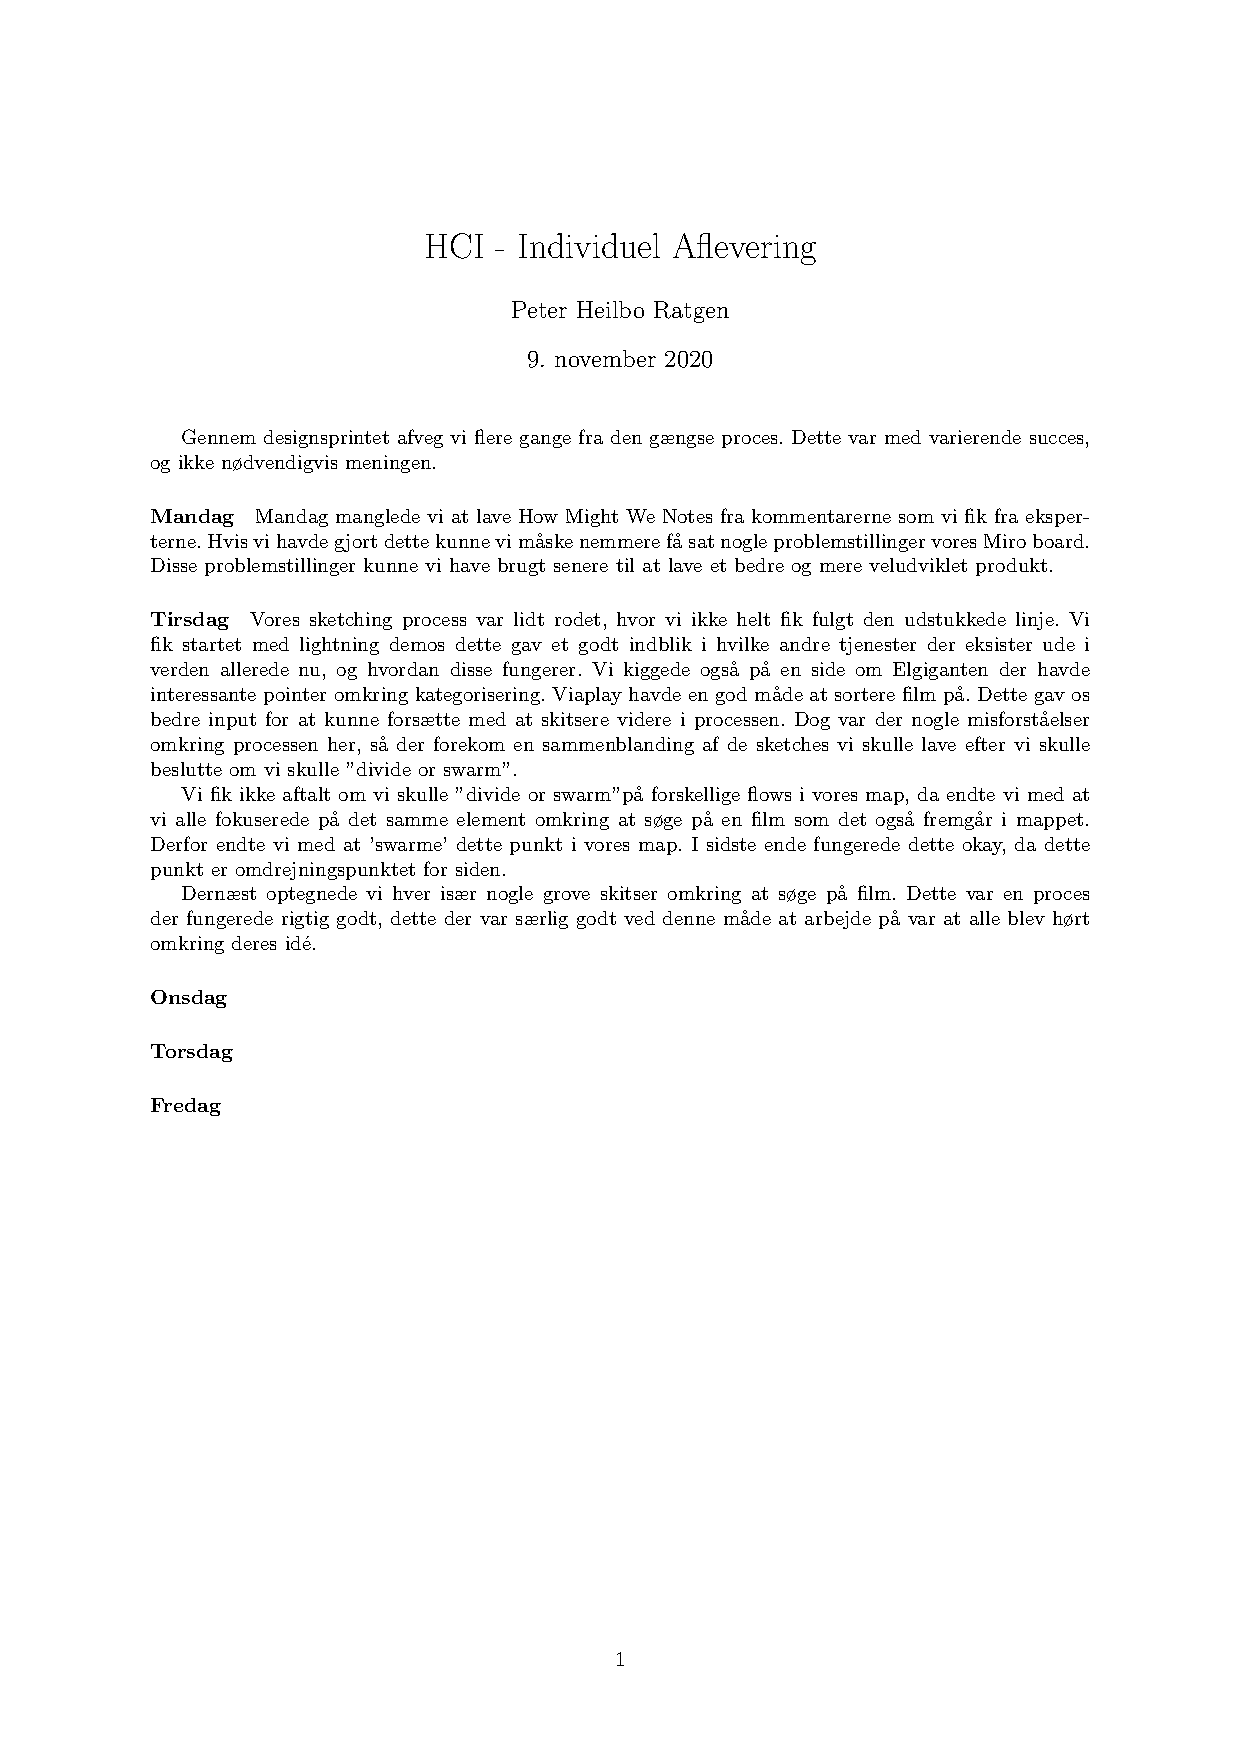
\includegraphics[width=0.5\textwidth]{./assignment/assignment.pdf}
\end{figure}

\end{document}
